\documentclass[11pt]{amsart}
\usepackage{amsmath}
\usepackage{amssymb}
\usepackage{tikz}
\usetikzlibrary{matrix,backgrounds}

\begin{document}

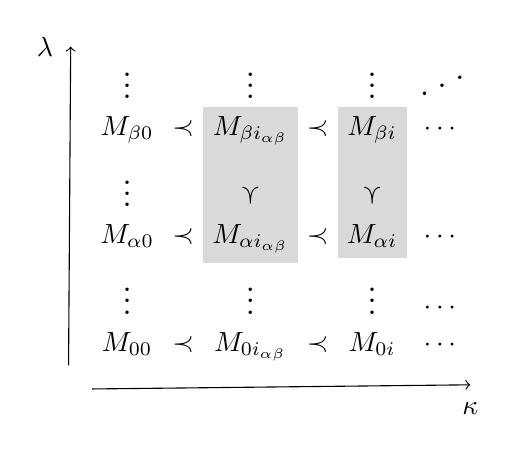
\begin{tikzpicture}[font=\ttfamily,
array1/.style={matrix of nodes}]

\matrix[array1] (array1) {
	$\vdots$ & & $\vdots$ & & $\vdots$ & \reflectbox{$\ddots$}\\
$M_{\beta 0}$ & $\prec$ & $M_{\beta i_{\alpha\beta}}$ & $\prec$ & $M_{\beta i}$ & $\cdots$\\
 $\vdots$& & \rotatebox{90}{$\prec$} & & \rotatebox{90}{$\prec$} &\\
$M_{\alpha 0}$ & $\prec$ & $M_{\alpha i_{\alpha\beta}}$ & $\prec$ & $M_{\alpha
i}$ & $\cdots$\\
 $\vdots$& & $\vdots$ & & $\vdots$
 & $\cdots$\\
$M_{00}$ & $\prec$ & $M_{0 i_{\alpha\beta}}$ & $\prec$ & $M_{0 i}$ & $\cdots$\\};
%
\draw[->]([yshift=-3mm]array1-6-1.south west) --
([yshift=-3mm]array1-6-6.south east);

\begin{scope}[on background layer]
\fill[gray!30] (array1-2-3.north west) rectangle (array1-4-3.south east);
\fill[gray!30] (array1-2-5.north west) rectangle (array1-4-5.south east);
\end{scope}

\draw[->]([xshift=-3mm]array1-6-1.south west) --
([xshift=-5mm]array1-1-1.north west);
\node [anchor=east] at ([xshift=-6mm]array1-1-1.north west) (k) {$\lambda$};
\node [anchor=north] at ([yshift=-4mm]array1-6-6.south east) (l) {$\kappa$};
%
\end{tikzpicture}

\end{document}